\documentclass[a4paper]{article}

\usepackage[margin=1.0in]{geometry}
\usepackage{amsmath}
\usepackage[table]{xcolor}
\usepackage{longtable}
\usepackage{fancyhdr}
\usepackage[auto-lang=false]{lipsum}
\usepackage{booktabs}
\usepackage{tikz}
\usetikzlibrary{backgrounds}

\setlength{\arrayrulewidth}{0.5mm}
\setlength{\tabcolsep}{18pt}
\renewcommand{\arraystretch}{1.5}

\begin{document}

    \begin{titlepage}

        \begin{center}
            \vspace*{1cm}

            \Huge
            \textbf{MAT 352 Assignment --- 2}

            \vspace{1.5cm}

            \textbf{Computer Science Department}

            \vspace{2cm}
            \normalsize
            \raggedright{
            \section*{Question}
            \textbf{Prove that:}
            \begin{enumerate}
                \item $0 \leq P(A) \leq 1$
                \item $P[(A \cap B) \cup (A \cap C) \cup (B \cap C)] = P(A \cap B) + P(A \cap C) + P(B \cap C) - 2P(A \cap B \cap C)$
                \item $P(x=x) = q^{x-1}p$ where $x=1,2,\ldots$ and $q = 1-p$
            \end{enumerate}}

            \vspace{5cm}
            \centering
            Submitted to Dr.\ Adinya

            \vspace{1cm}
            \today
        \end{center}

    \end{titlepage}

    \pagenumbering{arabic}
	\pagestyle{fancy}
	\fancyhead{}
	\fancyhead[L]{\textbf{MAT 352 Assignment}}
	\fancyhead[R]{\textbf{Computer Science}}

    \section*{Name of Students}
    \begin{center}
        \rowcolors{4}{gray}{lightgray}
        \Large
        \begin{longtable} { c|l|c }
            \toprule[2pt]
            S/N & \multicolumn{1}{|c|}{Name} & Matric Number \\
            \midrule
            1 & Adebowale Joseph Akintomiwa & 214846\\
            2 & Adedapo Anjorin & 214864\\
            3 & Adegbola Olatunde Williams & 207186\\
            4 & Adeleke Sherifdeen Adeboye & 214848\\
            5 & Adeleke Timothy Toluwani & 214849\\
            6 & Adelowo Samuel Damilare & 214850\\
            7 & Adeoti Warith Adetayo & 214851\\
            8 & Adim Chimaobi Solomon & 222455\\
            9 & Adisa Inioluwa Christiana & 214853\\
            10 & Ahmad Animasaun & 214863\\
            11 & Ajayi Prince Ayokunle & 215221\\
            12 & Akinade Faith Eniola & 222459\\
            13 & Akinrinola Akinfolarin & 205526\\
            14 & Akinrinola, Blessing Opemipo & 214857\\
            15 & Akinwusi Ifeoluwa & 214858\\
            16 & Alao Tawakalit Omowunmi & 222461\\
            17 & Alatise Oluwaseun Abraham & 214860\\
            18 & Arowolo Ayomide Stephen & 214865\\
            19 & Brai Daniel & 214868\\
            20 & Chinedu Promise Okafor & 213930\\
            21 & Daniel Emmanuel Oghenetega & 224870\\
            22 & Denedo Oghenetega & 214873\\
            23 & Emiade James & 214874\\
            24 & Farayola Joshua Olatunde & 214878\\
            25 & Godwin Daniel & 214871\\
            26 & Ibraheem Nuh Babatunde & 214879\\
            27 & Ikwuegbu Michael & 214881\\
            28 & Kareem Mustapha Babatunde & 214883\\
            29 & Kayode Peter Temitope & 208077\\
            30 & Kehinde Boluwatife Soyoye & 214916\\
            31 & Kip Charles Okechukwu Emeka & 215061\\
            32 & Matric  & Number\\
            33 & Kubiat Laura & 214884\\
            34 & Lawal Uchechukwu Adebayo & 214885\\
            35 & Matthews Victoria Olayide & 214886\\
            36 & Nwatu Chidinma Augustina & 214890\\
            37 & Odulate Oluwatobi Gabriel & 214893\\
            38 & Ogbolu Precious Chiamaka & 214894\\
            39 & Oghie Daniel O. & 214895\\
            40 & Ogunesan Rhoda Oluwatosin & 214897\\
            41 & Ogunyemi Temidayo Samuel & 214898\\
            42 & Ojewale Opeoluwa David & 214899\\
            43 & Okafor Lisa Chisom & 214901\\
            44 & Okoro Joshua Akachukwu & 214902\\
            45 & Okumagba Oghenerukevwe Miracle & 222498\\
            46 & Olagidi Joshua & 222500\\
            47 & Olalere Khadijat Titilayo & 222502\\
            48 & Olatunji Michael Oluwayemi & 214903\\
            49 & Olawale Eniola Emmanuel & 214904\\
            50 & Olorogun Ebikabowei Caleb & 214906\\
            51 & Oluwatade Iyanuoluwa & 214907\\
            52 & Oluwayelu Oluwanifise & 215257\\
            53 & Onasoga Oluwapelumi Idris & 214909\\
            54 & Oyekanmi Eniola & 214913\\
            55 & Sadiq Peter & 214914\\
            56 & Salami Lateefat Abimbola & 214915\\
            57 & Stephen Chidiebere Ivuelekwa & 214882\\
            58 & Toluwanimi Oluwabukunmi Osuolale & 214912\\
            59 & Ubaka Amazing-Grace Onyiyechukwu & 214918\\
            60 & Uchechukwu Ahunanya & 214854\\
            61 & Wisdom Oyor & 215206\\
            \bottomrule[4pt]
        \end{longtable}
        \normalsize
    \end{center}

    \newpage

    \section{Proof that $0 \leq P(A) \leq 1$}

    Let $S$ be a sample space and $A$ be an event defined on the sample space $S$

    \paragraph*{Recall the Axioms of Probability:}
    \begin{itemize}
        \item Axiom 1: For any event $A$ of a sample space, $P(A) \ge 0$
        \item Axiom 2: For any sample space $S$, $P(S) = 1$
    \end{itemize}

    \subsection*{Proof:}
    Let $A^C = S \setminus A$ (Complement of event $A$) and since $A$ and $A^C$ are mutually exclusive (i.e both events cannot occur simultaneously) therefore:
    \begin{align}
        S &= A \cup A^C\\
        P(S) &= P(A) + P(A^C)\\
        P(A) &= P(S) - P(A^C) \label{equa}
    \end{align}
    From equation ({\ref{equa}}) above, it can be seen that $P(A) \le P(S)$. By Axiom 2 ($P(S) = 1$) therefore:
    \begin{align}
        P(A) &\le P(S)\\
        P(A) &\le 1 \label{uneq1}
    \end{align}
    By Axiom 1 ($P(A) \ge 0$) then:
    \begin{align} \label{uneq2}
        0 &\le  P(A)
    \end{align}
    Combining the inequalities (\ref{uneq1}) and (\ref{uneq2}) therefore:
    \begin{align}
        0 \le P(A) \le 1
    \end{align}

    \subsection*{Alternatively:}
    By definition, the probability of an event $A$ is the number of times $m$ it is found (or it occured) within the total number $n$ of possibilities.
    \begin{align} \label{pp_form}
        P(A) = \frac{m}{n}
    \end{align}
    Event $A$ may not be found at in all the total possibilities (i.e $m = 0$). It may also be found any number of times between $0$ and $n$ (i.e  $0 < m < n$) and finally, it may be found exactly $n$ number of times (i.e $m = n$). Therefore yielding the bound for $m$ as:
    \begin{align} \label{pp_l}
        0 \le m \le n
    \end{align}
    Dividing the inequality (\ref{pp_l}) above through by $n$ gives:
    \begin{align}
        \frac{0}{n} \le &\frac{m}{n} \le \frac{n}{n} \notag \\
        0 \le &\frac{m}{n} \le 1 \label{pp_m}
    \end{align}
    Substituting equation (\ref{pp_form}) in the inequality (\ref{pp_m}) above:
    \begin{align*}
        0 \le P(A) \le 1
    \end{align*}

    \newpage
    \section{Proof that $P[(A \cap B) \cup (A \cap C) \cup (B \cap C)] = P(A \cap B) + P(A \cap C) + P(B \cap C) - 2P(A \cap B \cap C)$}
    The proof can be shown by using the Inclusion-Exclusion Rule for any $n$ number of events which states that:
    \begin{equation} \label{i_e_rule}
        \begin{split}
            P(E_1 \cup E_2 \cup E_3 \cup \dots \cup E_n) = & \sum_{i = 1}^{n} P(E_i) - \sum_{i_1 < i_2} P(E_{i_1} \cap E_{i_2}) + \sum_{i_1 < i_2 < i_3} P(E_{i_1} \cap E_{i_2} \cap E_{i_3}) + \cdots + \\
            & {(-1)}^{r + 1} \sum_{i_1 < i_2 < \cdots < i_r} P(E_{i_1} \cap E_{i_2} \cap \cdots \cap E_{i_r}) + \cdots + \\
            & {(-1)}^{n} \sum_{i_1 < i_2 < \cdots < i_{n-1}} P(E_{i_1} \cap E_{i_2} \cap \cdots \cap E_{i_{n-1}}) + \\
            & {(-1)}^{n + 1} P(E_1 \cap E_2 \cap E_3 \cap \cdots \cap E_n)
        \end{split}
    \end{equation}
    Therefore:
    \begin{align}
        \begin{split} \label{equ_IE}
            P([A \cap B] \cup [A \cap C] \cup [B \cap C]) = & P(A \cap B) + P(A \cap C) + P(B \cap C) - P([A \cap B] \cap [A \cap C]) \\
            & - P([A \cap B] \cap [B \cap C]) - P([A \cap C] \cap [B \cap C]) \\
            & + P([A \cap B] \cap [A \cap C] \cap [B \cap C])
        \end{split}
    \end{align}
    From Set Theory:
    \begin{align*}
        &P([A \cap B] \cap [A \cap C])  = P(A \cap B \cap C) \\
        &P([A \cap B] \cap [A \cap C] \cap [B \cap C]) = P(A \cap B \cap C)
    \end{align*}
    This is illustrated using the Venn diagram below

    \begin{center}
        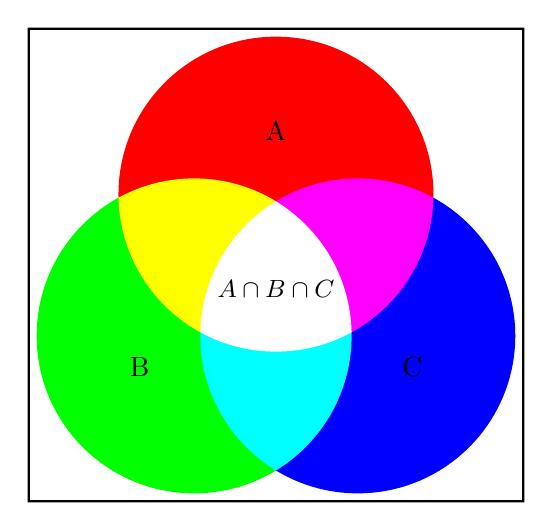
\begin{tikzpicture}
            \begin{scope}[blend group=screen, framed]
                \fill[red]   ( 90:1.2) circle (2);
                \fill[green] (210:1.2) circle (2);
                \fill[blue]  (330:1.2) circle (2);
                \draw[thick] ([shift={(-0.1,-0.1)}]current bounding box.south west) rectangle ([shift={(0.1,0.1)}]current bounding box.north east);
            \end{scope}
            \node at ( 90:2)    {A};
            \node at (210:2)    {B};
            \node at (330:2)    {C};
            \node [font=\small] {$A \cap B \cap C$};
        \end{tikzpicture}
    \end{center}

    \begin{itemize}
        \item $[A \cap B] \cap [A \cap C]$: $[A \cap B]$ includes the yellow and the white regions and $[A \cap C]$ is the purple and the white regions. The region common to both is the white region ($A \cap B \cap C$)
        \item $[A \cap B] \cap [B \cap C]$: $[A \cap B]$ includes the yellow and the white regions and $[B \cap C]$ is the cyan and the white regions. The region common to both is the white region ($A \cap B \cap C$)
        \item $[A \cap C] \cap [B \cap C]$: $[A \cap C]$ includes the purple and the white regions and $[B \cap C]$ is the cyan and the white regions. The region common to both is the white region ($A \cap B \cap C$)
        \item $[A \cap B] \cap [A \cap C] \cap [B \cap C]$: $[A \cap B] = \text{yellow and white region}$, $[A \cap C] = \text{purple and white region}$, $[B \cap C] = \text{cyan and white region}$. Common to all three regions is the white region ($A \cap B \cap C$)
    \end{itemize}
    Equation (\ref{equ_IE}) is the simplified as:
    \begin{align}
        \begin{split}
            P([A \cap B] \cup [A \cap C] \cup [B \cap C]) = & P(A \cap B) + P(A \cap C) + P(B \cap C) - P(A \cap B \cap C) \\
            & - P(A \cap B \cap C) - P(A \cap B \cap C) + P(A \cap B \cap C)
        \end{split} \\
        \begin{split}
            = & P(A \cap B) + P(A \cap C) + P(B \cap C) \\
            & - P(A \cap B \cap C) - P(A \cap B \cap C)
        \end{split}
    \end{align}
    Finally:
    \begin{align}
        P([A \cap B] \cup [A \cap C] \cup [B \cap C]) = P(A \cap B) + P(A \cap C) + P(B \cap C) - 2P(A \cap B \cap C)
    \end{align}

    \vspace{1cm}
    \section{Proof that $P(x=x) = q^{x-1}p$ where $x=1,2,\ldots$ and $q = 1-p$}
    The proof for this formular can be shown by \textbf{Axiom 2} of the probability theory that:
    \begin{equation}P(S) = 1\end{equation}
    where $S$ is the sample space.

    \paragraph*{Given that $X$ is a random variable with $X \in \{1, 2, \ldots\}$ and $q = 1 - p$}

    \begin{align}
        P(S) &= P(X=1) + P(X=2) + P(X=3) + \cdots\\
        &= q^{1-1}p + q^{2-1}p + q^{3-1}p + \cdots\\
        &= q^{0}p + q^{1}p + q^{2}p + \cdots\\
        &= p + qp + q^{2}p + \cdots \label{q_sum}
    \end{align}
    The equation above shows an infinite geometric sum where: $a_1 = p$, $a_2 = qp$, $a_3 = q^{2}p$, $\ldots$ and the common ratio $r = q$

    The sum of infinite geometric series is given by:

    \begin{align*}
        S_n = a_1 + a_2 + a_3 + \cdots &= \sum_{i=1}^{\infty}a_i\\
        &= \frac{a}{1 - r}
    \end{align*}
    Therefore, we can simplify (\ref{q_sum}) by using the geometric sum and substituting $q = 1 - p$.

    \begin{align*}
        P(S) &= p + qp + q^{2}p + \cdots\\
        &= \frac{p}{1 - q}\\
        &= \frac{p}{1 - (1 - p)}\\
        &= \frac{p}{1 - 1 + p}\\
        &= \frac{p}{p}\\
        &= 1
    \end{align*}
    So, $P(S) = \sum_{i=1}^{\infty}P[X=x] = \sum_{i=1}^{\infty}q^{x-1}p = 1$.

    \paragraph*{Therefore it is true that $P[X=x] = q^{x-1}p$ where $x = 1, 2, \ldots$ and $q = 1 - p$}


\end{document}
